\section{Auswertung}

\subsection{statische Methode \label{sec:stat}}

In den Abbildungen \ref{fig:stat1} und \ref{fig:stat2} sind die aufgenommenen Messwerte dargestellt.
\begin{figure}[H]
  \centering
  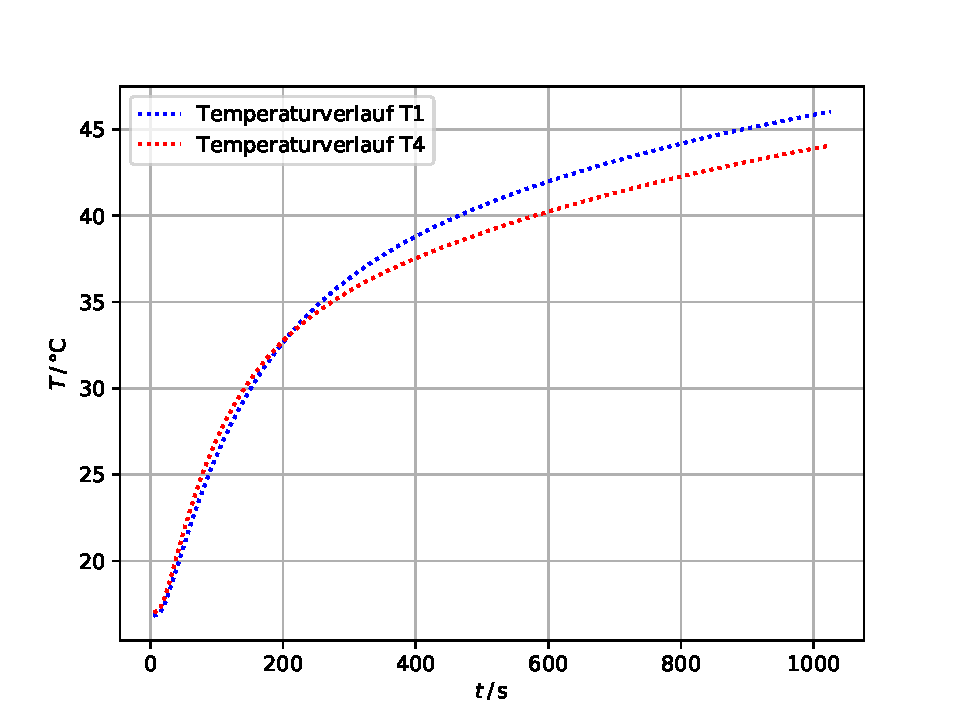
\includegraphics[width=\textwidth]{Plots/stat1.pdf}
  \caption{$T$-$t$-Diagramm mit den Temperaturverläufen am breiten ($T1$) und schmalen ($T4$) Messingstab}
  \label{fig:stat1}
\end{figure}
\begin{figure}[H]
  \centering
  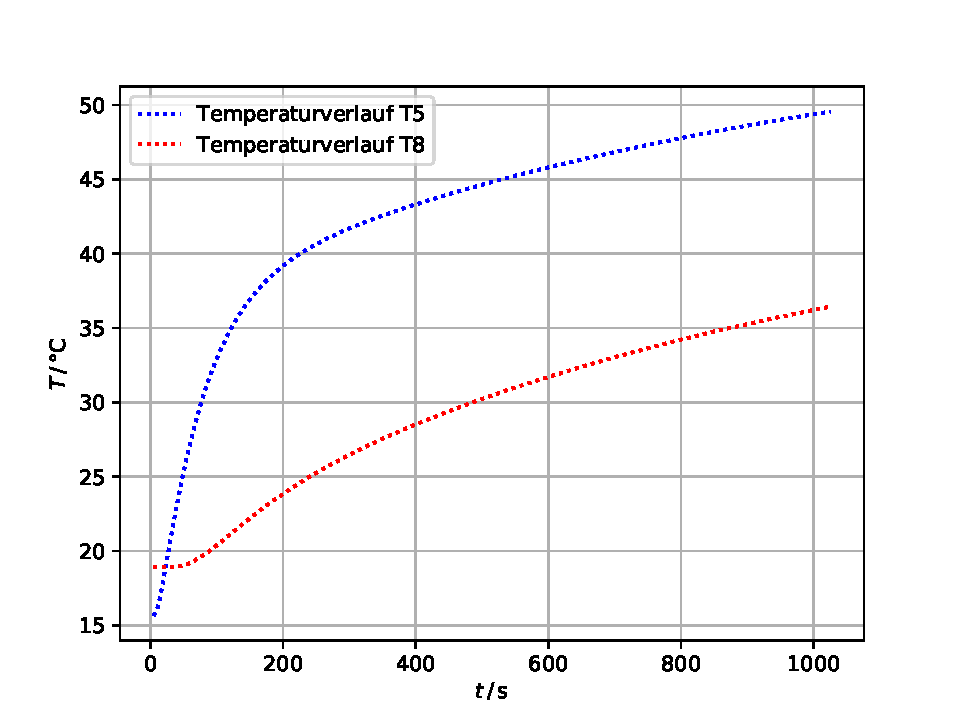
\includegraphics[width=\textwidth]{Plots/stat2.pdf}
  \caption{$T$-$t$-Diagramm mit den Temperaturverläufen am Aluminium- ($T5$) und Edelstahlstab ($T8$)}
  \label{fig:stat2}
\end{figure}

Die nach $\SI{700}{\s}$ aufgenommenen Temperaturen betragen
\begin{align*}
  T_1 &= \SI{43,16}{°C} \\
  T_4 &= \SI{41,32}{°C} \\
  T_5 &= \SI{46,84}{°C} \\
  T_8 &= \SI{33,04}{°C}
\end{align*}

Die vier Graphen zeigen jeweils einen logarithmischen Verlauf. Der stärkste Anstieg findet dabei
in der Zeit bis ungefähr $\SI{200}{\s}$ satt.
Dabei streben die Graphen unterschiedlichen Temperaturen zu.
Außerdem ist zu erkennen, dass Aluminium die höchste Wärmeleitfähigkeit besitzt und Edelstahl die niedrigste.
Desweiteren ist die Wärmeleitung bei größerer Fläche größer, wie beim Vergleich von $T1$ und $T4$ auffällt.

In der Abbildung \ref{fig:diff} sind die Temperaturdifferenzen dargestellt.
\begin{figure}[H]
  \centering
  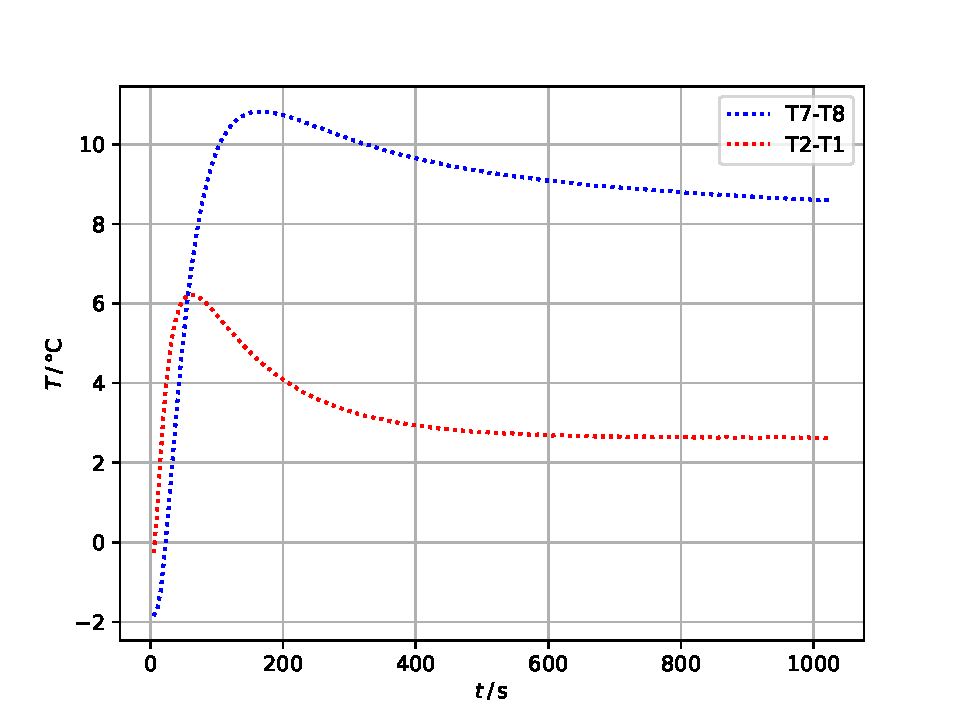
\includegraphics[width=\textwidth]{Plots/diff.pdf}
  \caption{$T$-$t$-Diagramm mit den Temperaturdifferenzen am breiten Messingstab ($T2 - T1$) und Edelstahlstab ($T7 - T8$).}
  \label{fig:diff}
\end{figure}

Auffällig ist hier, dass beide Graphen einen zunächst starken Anstieg haben und nach dem erreichen eines Maximums
auf einen konstanten Wert fallen.
Der Messingstab erreicht dabei sein Maximum bei $\SI{6}{°C}$ nach ungefähr $\SI{50}{\s}$ und fällt
im Anschluss auf knapp $\SI{3}{°C}$. Der Edelstahlstab braucht mit ca. $\SI{150}{\s}$ dreimal so lange,
um sein Maximum zu erreichen, das bei über $\SI{10}{°C}$ liegt. Der konstante Wert, der sich danach einstellt,
ist mit knapp $\SI{9}{°C}$ auch dreimal so hoch wie beim Messingstab.
Hieraus lässt sich ebenfalls darauf schließen, dass Edelstahl eine viel geringere Wärmeleitfähigkeit als
Messing besitzt, da die Temperaturdifferenzen zwischen den beiden Thermoelementen größer ist.
Das heißt, dass die Wärme langsamer transportiert wird.

Mit Gleichung \eqref{eqn:dQ} soll für fünf unterschiedliche Zeiten der Wärmestrom $\Phi = \frac{\Delta Q}{\Delta t}$
berechnet werden. Die Ergebnisse befinden sich in Tabelle \ref{tab:qstrom}.
Der Abstand zwischen den Thermoelementen ist $\Delta x = \SI{30}{\centi \meter}$ und die Wärmeleitfähigkeiten
\cite{sample2} von Messing und Edelstahl betragen
\begin{align*}
  \kappa_\text{theo, Messing} &= \SI{109}{\watt \per \meter \per \kelvin} \\
  \kappa_\text{theo, Edelstahl} &= \SI{16}{\watt \per \meter \per \kelvin}
\end{align*}

\begin{table}[H]
  \centering
  \caption{Wärmestrom von Messing und Edelstahl}
  \label{tab:qstrom}
  \begin{tabular}{c S S}
    \toprule
      {$t \:/\: \mathrm{s}$}  & {$\Phi_\text{Messing} \:/\: \mathrm{W}$} &
      {$\Phi_\text{Edelstahl} \:/\: \mathrm{W}$}\\
    \midrule
       100  & -1,00 & -0,25 \\
       300  & -0,58 & -0,26 \\
       500  & -0,48 & -0,24 \\
       700  & -0,46 & -0,23 \\
       900  & -0,46 & -0,22 \\
    \bottomrule
  \end{tabular}
\end{table}

\subsection{Dynamische Methode}

\subsubsection{Breiter Messingstab}

Die aufgenommenen Messwerte sind in Abbildung \ref{fig:mesdyn} aufgetragen.
\begin{figure}[H]
  \centering
  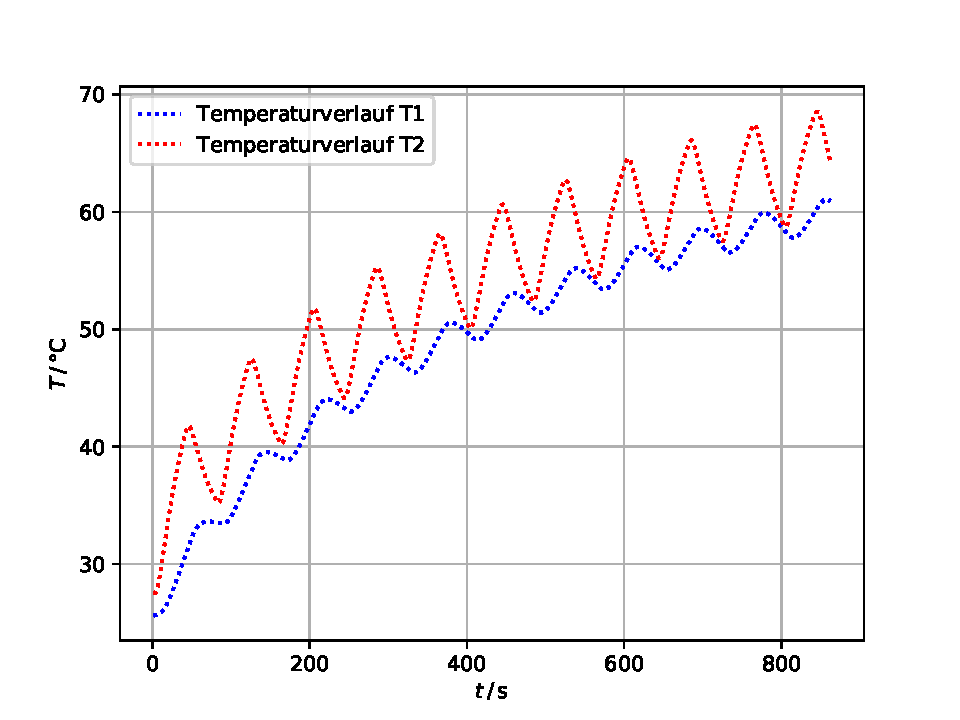
\includegraphics[width=\textwidth]{Plots/mesdyn.pdf}
  \caption{$T$-$t$-Diagramm mit den Temperaturverläufen $T1$ und $T2$ am breiten Messingstab
            bei einer Periode von $\SI{80}{\s}$.}
  \label{fig:mesdyn}
\end{figure}

Die daraus bestimmten Amplituden und Phasendifferenzen befinden sich in Tabelle \ref{tab:mesdyn}.
\begin{table}[H]
  \centering
  \caption{Werte zur Bestimmung der Wärmeleitfähigkeit von Messing}
  \label{tab:mesdyn}
  \begin{tabular}{c c c c}
    \toprule
       & {$A_\text{nah} \:/\: \mathrm{K}$}  & {$A_\text{fern} \:/\: \mathrm{K}$} &
      {$\Delta t \:/\: \mathrm{s}$}\\
    \midrule
     & 10,3 & 3,0 & 18 \\
     & 10,0 & 2,9 & 16 \\
     & 9,7 & 3,0 & 16 \\
     & 9,7 & 2,9 & 16 \\
     & 9,5 & 2,7 & 14 \\
     & 9,4 & 2,7 & 16 \\
     & 9,5 & 2,9 & 16 \\
     & 9,5 & 2,9 & 14 \\
     & 9,4 & 2,7 & 11 \\
     & 9,4 & 2,9 & 14 \\
     Mittelwert & 9,64 \pm 0,09 & 2,86 \pm 0,04 & 15,1 \pm 0,6 \\
    \bottomrule
  \end{tabular}
\end{table}

Die Mittelwerte errechnen sich dabei aus
\begin{equation}
  \bar{x} = \frac{1}{N} \sum_{i=1}^{N} x_i
  \label{eqn:mit}
\end{equation}

und die Standardabweichungen aus
\begin{equation}
  \Delta \bar{x} = \sqrt{\frac{1}{N (N - 1)} \sum_{i=1}^{N} (x_i - \bar{x})^2}.
  \label{eqn:sta}
\end{equation}

Mithilfe von Gleichung \eqref{eqn:kap} und der Gauß'schen Fehlerfortpflanzung
\begin{equation}
  \delta = \sqrt{ \sum_{i=1}^{n}(\frac{\partial y}{\partial x_i} \Delta x_i)^2}
  \label{eqn:gaus}
\end{equation}

ergibt sich für die Wärmeleitfähigkeit
\begin{equation*}
  \kappa_\text{Messing} = \SI{80,45(340)}{\watt \per \meter \per \kelvin}.
\end{equation*}

Die Abweichung vom Theoriewert $\kappa_\text{theo, Messing} = \SI{109}{\watt \per \meter \per \kelvin}$ beträgt
$26,19 \%$.

\subsubsection{Aluminiumstab}
Die aufgenommenen Messwerte sind in Abbildung \ref{fig:aludyn} aufgetragen.
\begin{figure}[H]
  \centering
  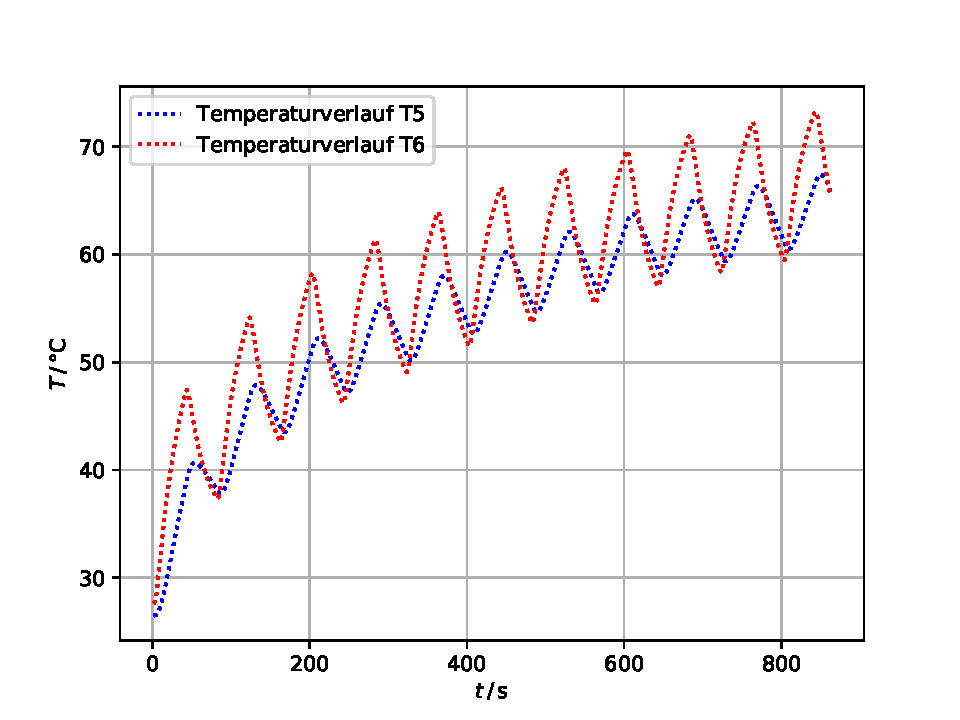
\includegraphics[width=\textwidth]{Plots/aludyn.pdf}
  \caption{$T$-$t$-Diagramm mit den Temperaturverläufen $T5$ und $T6$ am Aluminiumstab
            bei einer Periode von $\SI{80}{\s}$.}
  \label{fig:aludyn}
\end{figure}

Die daraus bestimmten Amplituden und Phasendifferenzen befinden sich in Tabelle \ref{tab:aludyn}.
\begin{table}[H]
  \centering
  \caption{Werte zur Bestimmung der Wärmeleitfähigkeit von Aluminium}
  \label{tab:aludyn}
  \begin{tabular}{c c c c}
    \toprule
       & {$A_\text{nah} \:/\: \mathrm{K}$}  & {$A_\text{fern} \:/\: \mathrm{K}$} &
      {$\Delta t \:/\: \mathrm{s}$}\\
    \midrule
     & 13,8 & 7,3 & 14 \\
     & 13,0 & 6,7 & 14 \\
     & 12,9 & 6,4 & 14 \\
     & 12,7 & 6,4 & 12 \\
     & 12,6 & 6,2 & 12 \\
     & 12,6 & 6,2 & 12 \\
     & 12,4 & 6,2 & 12 \\
     & 12,4 & 6,2 & 14 \\
     & 12,4 & 6,1 & 12 \\
     & 12,4 & 6,1 & 12 \\
     Mittelwert & 12,72 \pm 0,14 & 6,38 \pm 0,12 & 12,8 \pm 0,3 \\
    \bottomrule
  \end{tabular}
\end{table}

Die Mittelwerte und Standardabweichungen ergeben sich aus den Gleichungen \eqref{eqn:mit} und \eqref{eqn:sta}.
Mithilfe von Gleichung \eqref{eqn:kap} und der Gauß'schen Fehlerfortpflanzung \eqref{eqn:gaus}
ergibt sich für die Wärmeleitfähigkeit
\begin{equation*}
  \kappa_\text{Aluminium} = \SI{118,41(475)}{\watt \per \meter \per \kelvin}.
\end{equation*}

Die Abweichung vom Theoriewert $\kappa_\text{theo, Aluminium} = \SI{205}{\watt \per \meter \per \kelvin}$
\cite{sample2} beträgt $42,24 \%$.

\subsubsection{Edelstahlstab}
Die aufgenommenen Messwerte sind in Abbildung \ref{fig:edeldyn} aufgetragen.
\begin{figure}[H]
  \centering
  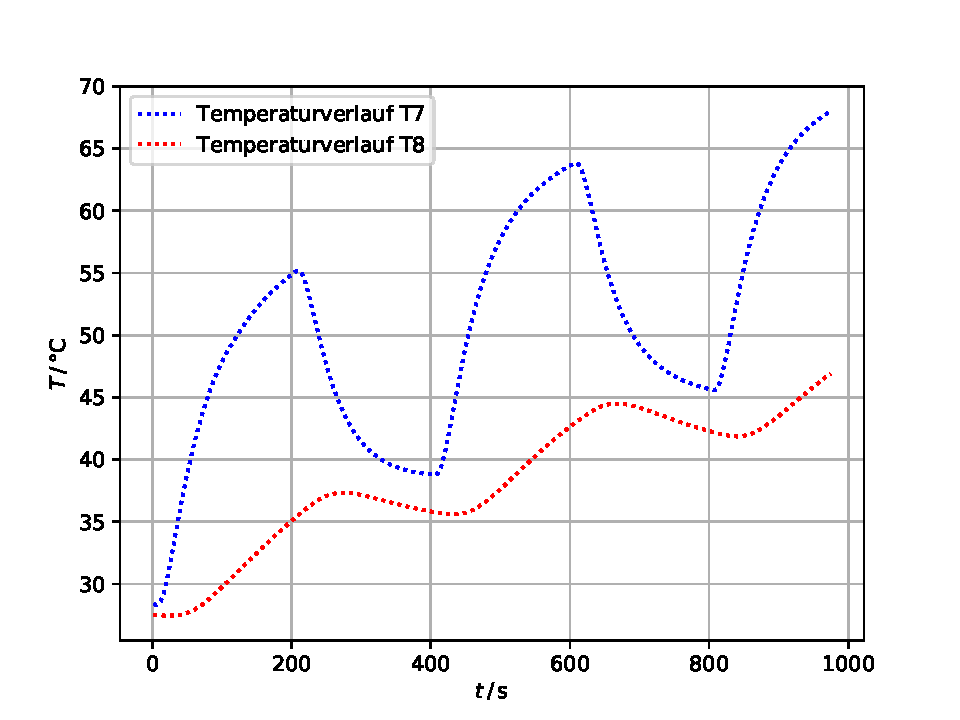
\includegraphics[width=\textwidth]{Plots/edeldyn.pdf}
  \caption{$T$-$t$-Diagramm mit den Temperaturverläufen $T7$ und $T8$ am Edelstahlstab
            bei einer Periode von $\SI{200}{\s}$.}
  \label{fig:edeldyn}
\end{figure}

Die daraus bestimmten Amplituden und Phasendifferenzen befinden sich in Tabelle \ref{tab:edeldyn}.
\begin{table}[H]
  \centering
  \caption{Werte zur Bestimmung der Wärmeleitfähigkeit von Edelstahl}
  \label{tab:edeldyn}
  \begin{tabular}{c c c c}
    \toprule
       & {$A_\text{nah} \:/\: \mathrm{K}$}  & {$A_\text{fern} \:/\: \mathrm{K}$} &
      {$\Delta t \:/\: \mathrm{s}$}\\
    \midrule
     & 22,0 & 5,4 & 62 \\
     & 21,9 & 5,6 & 60 \\
     Mittelwert & 21,95 \pm 0,05 & 5,50 \pm 0,10 & 61,0 \pm 1,0 \\
    \bottomrule
  \end{tabular}
\end{table}

Die Mittelwerte und Standardabweichungen ergeben sich aus den Gleichungen \eqref{eqn:mit} und \eqref{eqn:sta}.
Mithilfe von Gleichung \eqref{eqn:kap} und der Gauß'schen Fehlerfortpflanzung \eqref{eqn:gaus}
ergibt sich für die Wärmeleitfähigkeit
\begin{equation*}
  \kappa_\text{Edelstahl} = \SI{17,06(36)}{\watt \per \meter \per \kelvin}.
\end{equation*}

Die Abweichung vom Theoriewert $\kappa_\text{theo, Edelstahl} = \SI{16}{\watt \per \meter \per \kelvin}$
beträgt $6,63 \%$.
